\vorlesung{25. Januar 2018}

\chapter{Die Schwache Wechselwirkung}
Bisher haben wir gesehen:
\begin{itemize}
\item $\beta$-Zerfälle von Kernen
\item Hadron-Zerfälle
\item Neutrinos
\end{itemize}
\tb{Jetzt: }Systematisch
\section{Grundlegende Struktur}
\begin{itemize}
\item WW durch Austausch von Bosonen (wie QED, QCD)
\item Austauschteilchen sind massiv und geladen:\\
$W^\pm$, $M_W = 80.4\,$GeV\\
$Z^0$, $M_Z = 91.2$\,GeV
\item koppelt an \tb{alle} Fermionen (einzige WW von Neutrinos)
\item Immer: $W$- oder $Z$-Propagator
\begin{align}
\boxed{\mc{M} \sim \frac{1}{Q^2 + M_{W,Z}^2} \, \Ra \, \sigma,\ \Gamma \overset{Q^2 \ll M_{W,Z}^2}{\sim} \frac{1}{M_{W,Z}^4}}
\end{align}
Nenner $M_{W,Z}^4$ ist der Grund dafür, warum die schwache WW schwach ist.
\item Eichstruktur (angedeutet)
\begin{align}
\underbrace{SU(2)\begin{pmatrix}\cdot\\ \cdot\end{pmatrix}_L}_{\substack{\text{Eichbosonen:}\\W^-, W^0, W^+}} \hspace*{1cm} \underbrace{U(1) (\cdot)_R}_{\substack{\text{Eichboson:}\\B}}
\end{align}
$SU(2)$ ist linkshändig, $U(1)$ dagegen rechtshändig.\\
Die Eichbosonen $W^0$ und $B$ können mischen. Es gilt dafür:
\begin{align}
\begin{pmatrix}
Z^0 \\ \gamma
\end{pmatrix} = \begin{pmatrix}
\cos \theta_W & - \sin \theta_W\\  \sin \theta_W & \cos \theta_W
\end{pmatrix} \begin{pmatrix}
W^0 \\ B
\end{pmatrix}
\end{align}
(\glqq elektroschwache Vereinigung\grqq{})
\begin{compactitem}
\item[mit] $\theta_W$: Weinberg-Winkel
\item[] $\sin^2 \theta_W \approx 0.222$
\item[] $\Ra$ $Z^0$ hat \glqq elektromagnetischen Anteil\grqq{}
\end{compactitem}
\item Higgs-Boson:\\
Notwendig, um massive Eichbosonen zu erklären, ohne Eichsymmetrie zu verletzen
\end{itemize}

\section{Der geladene Strom}

$W^\pm$-Austausch, koppelt an alle Fermionen:

\begin{figure}[!ht]
\centering
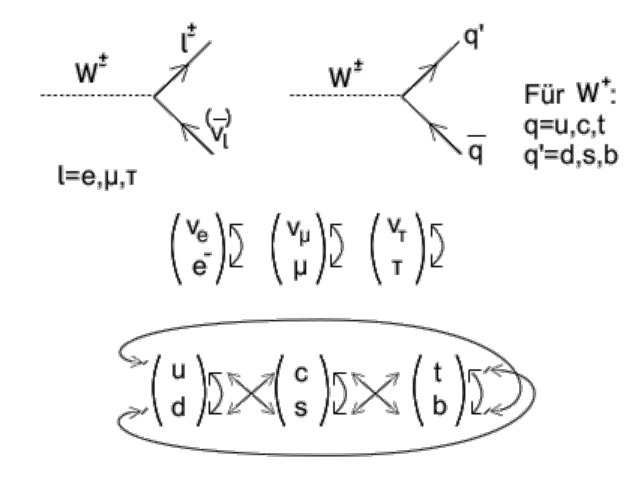
\includegraphics[width=.5\textwidth]{imgs/ep5-fig-8-1.pdf}
\caption{$W$-Kopplung an ein Lepton und das zugehörige Neutrino bzw. an ein Quark \label{fig:8.1}}
\end{figure}

\begin{itemize}
\item Kopplungsstärke
\begin{align}
g_W = \frac{e}{\sin \theta_W}
\end{align}
$\Ra$ \tb{stärker} als bei elm. WW!
\item \tb{Quark-Mischung}\\
Beobachtet z.B. bei Zerfall der leichtesten Mesonen/Baryonen mit $S\neq 0$

\begin{figure}[!ht]
\centering
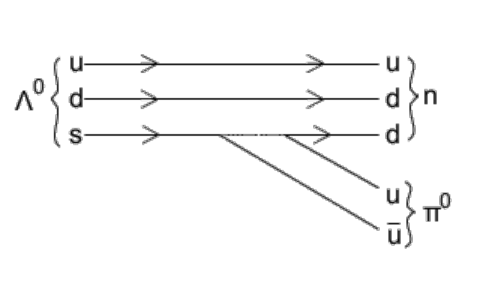
\includegraphics[width=.5\textwidth]{imgs/ep5-fig-8-2.pdf}
\caption{Quark-Mischung am Beispiel $\Lambda^0 \ra n \pi^0$\label{fig:8.2}}
\end{figure}
\newpage
Erklärung:
\begin{framed}
\begin{center}
Quark-EZ der schwachen WW $\neq$ Quark-EZ der starken WW
\end{center}
\end{framed}
QM: Beide EZ-Vektoren durch unitäre Transformation verknüpft. Für d,s ergibt sich:
\begin{align}
\boxed{ \underbrace{\begin{pmatrix}
d^\prime \\ s^\prime 
\end{pmatrix}}_\text{schwach} = \underbrace{\begin{pmatrix}
\cos \theta_C & \sin \theta_C\\ -\sin\theta_C & \cos \theta_C \end{pmatrix}}_\text{Cabibbo-Matrix} \underbrace{\begin{pmatrix}
d \\ s
\end{pmatrix}}_\text{stark}
 }
\end{align}
Hierbei ist $\theta_C$ der sogenannte Cabibbo-Winkel.
\begin{align*}
\sin \theta_C \approx 0.22, \sin^2 \theta_C \approx 0.05
\end{align*}
\begin{itemize}
\item[$\Ra$] Geladener Strom hat Terme:
\begin{align}
\begin{pmatrix}
u \\ c
\end{pmatrix}^\top U_\mr{Cab} \begin{pmatrix}
d \\ s
\end{pmatrix}=\quad \begin{cases}\quad 
\lno \begin{matrix}
ud \cdot \cos \theta_C & +\\ cs \cdot \cos\theta_C & +
\end{matrix} \rrb \labs \mc{M}\rabs^2 \sim \cos^2 \theta_C \approx 0.95\\ \ \\
\quad \lno \begin{matrix}
us \cdot \sin \theta_C & -\\ cd \cdot \sin\theta_C & -
\end{matrix} \rrb \labs \mc{M}\rabs^2 \sim \sin^2 \theta_C \approx 0.05 \end{cases}
\end{align}
\item[$\lt$] $U_\mr{Cab}$ kann auch als Mischung von $(u,c)$ interpretiert werden
\item[$\Ra$] \glqq Nicht diagonale\grqq{} Terme sind mit Faktor 20 unterdrückt.
\begin{figure}[!ht]
\centering
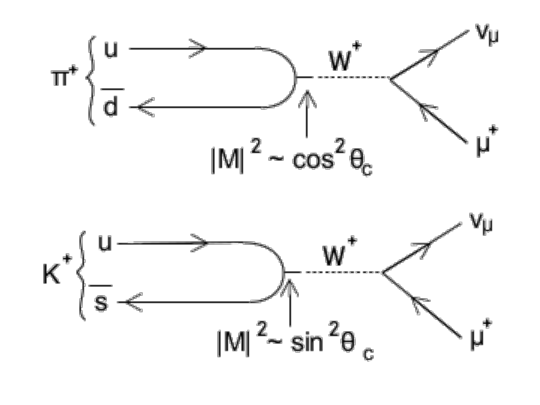
\includegraphics[width=.5\textwidth]{imgs/ep5-fig-8-3.pdf}
\caption{Offidiagonale ($\sin \theta_C$ Zerfälle unterdrückt \label{fig:8.3}}
\end{figure}

$\Ra$ Verallgemeinerung auf 3 Quark-Familien
\begin{align}
\boxed{ \begin{pmatrix}
d^\prime \\ s^\prime \\ b^\prime 
\end{pmatrix} = U(3) \cdot \begin{pmatrix}
d \\ s\\ b
\end{pmatrix} }
\end{align}
$U(3)$ = unitäre Matrix, genannt Cabibbo-Kobayashi-Maskawa-Matrix (CKMM)
\begin{itemize}
\item[$\lt$] 3 reelle Parameter (\glqq Drehwinkel\grqq{})
\item[$\lt$] komplexe Phase
\item[$\lt$] Beträge der Matrixelemente
\begin{align}
\begin{pmatrix}
0.974 & 0.225 & 0.004 \\
0.225 & 0.973 & 0.041\\
0.009 & 0.040 & 0.999
\end{pmatrix} \approx \begin{pmatrix}
U_\mr{Cab} & \begin{matrix}
0.004 \\ 0.041
\end{matrix} \\
\begin{matrix}
0.009 & 0.040
\end{matrix} & 0.999
\end{pmatrix}
\end{align}
sehr stark diagonaldominant
\item[$\ra$]  Aus unterer Zeile
\begin{align*}
\Gamma \lb  t \ra d\rb : \Gamma \lb t \ra s\rb  : \Gamma\lb t \ra b\rb  = (0.009)^2 : (0.040)^2 : (0.999)^2
\end{align*}

\begin{figure}[!ht]
\centering
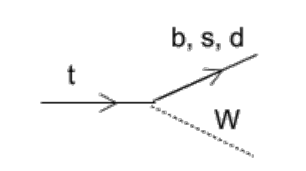
\includegraphics[width=.5\textwidth]{imgs/ep5-fig-8-4.pdf}
\caption{Feynmandiagramme zu WW bezüglich der unteren Zeile der CKMM \label{fig:8.4}}
\end{figure}
\end{itemize}
\end{itemize}
\end{itemize}
\section{Paritätsverletzung in der schwachen WW}
Erinnerung: Parität ist verletzt, wenn
\begin{align}\begin{split}
&\hat{P}^\dagger \Ham_{WW} \hat{P} \neq \Ham_{WW}\\
\Ra \mc{M}_P &= \braket{\Psi_f | \hat{P}^\dagger \Ham_{WW} \hat{P} | \Psi_i}\\
& = \braket{\hat{P}\Psi_f | \Ham_{WW} | \hat{P} \Psi_i}\\
& \neq \braket{\Psi_f | \Ham_{WW} | \Psi_i}
\end{split}\end{align}
raumgespiegelten Prozess $\neq$ Wahrscheinlichkeit für ungespiegelten Prozess.

Bis $\sim$1955: Fester \glqq Glaube\grqq{} an Paritätserhaltung.\\Dann: Experiment von C.S. Wu (1956)
\begin{align*}
\underset{\text{Spin 5}}{^{60}_{27} Co} \ra \underset{\text{Spin 4}}{^{60}_{28} Ni^\star} + e^- + \bar{\nu}_e
\end{align*}

\begin{figure}[!ht]
\centering
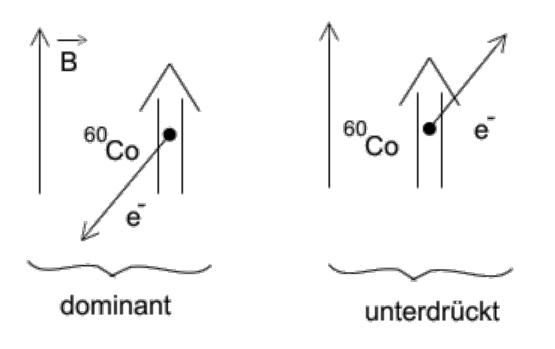
\includegraphics[width=.5\textwidth]{imgs/ep5-fig-8-5.pdf}
\caption{Experiment zur Paritätsverletzung bei schwacher WW\label{fig:8.5}}
\end{figure}
\newpage
Achtung: $\hat{P} \vec{B} = \vec{B}$, $\hat{P} \vec{J} = \vec{J}$, $\hat{P}\vec{p} = - \vec{p}$
\begin{itemize}
\item[$\Ra$] Paritätsverletzung!
\item[$\Ra$] Interpretation $\bar{\nu}$ ist rechtshändig, denn:

\begin{figure}[!ht]
\centering
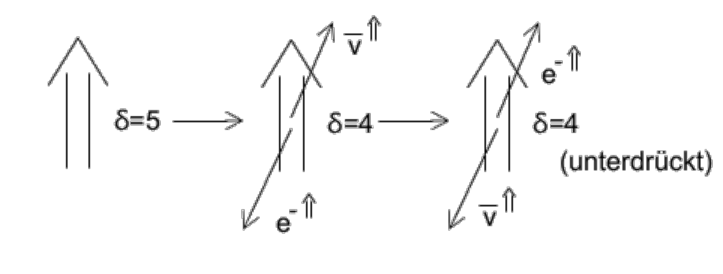
\includegraphics[width=.5\textwidth]{imgs/ep5-fig-8-6.pdf}
\caption{$\bar{\nu}$ ist rechtshändig, da die rechten Prozess unterdrückt ist \label{fig:8.6}}
\end{figure}
\item[$\Ra$] Schwache WW koppelt an linkshändige $\nu$'s und an rechtshändige $\bar{\nu}$'s\\
(1957 bestätigt in Goldhader-Experiment)

\begin{figure}[!ht]
\centering
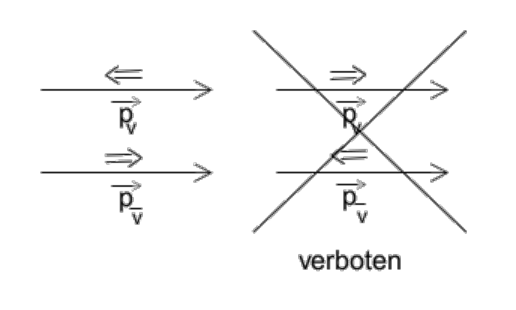
\includegraphics[width=.65\textwidth]{imgs/ep5-fig-8-7.pdf}
\caption{Skizze zum Goldhader-Experiment \label{fig:8.7}}
\end{figure}

\item[$\lt$] $\underbrace{\text{maximale}}_{\begin{pmatrix}
\nu_l\\l\end{pmatrix}_L, \ \begin{pmatrix}
q^\prime \\ q \end{pmatrix}_L}$ $\underbrace{\text{Paritätsverletzung!}}_{\substack{(l)_R, \ (q)_R\\\text{Koppeln nicht an $W$}}}$
\item[$\Ra$] Bisher: Helizität $h$
\begin{align}
h = \frac{\vec{\sigma}\vec{p}}{\labs \vec{\sigma}\rabs \labs \vec{p} \rabs}
\end{align}
In der Theorie der schwachen WW entscheiden \glqq Chiralität\grqq{} $\hat{C}_{L,R}$
\begin{align*}
\ket{\Psi} = \ket{\Psi_L} + \ket{\Psi_R} = \hat{C}_L \ket{\Psi} + \underbrace{\hat{C}_R}_{= (1-\hat{C}_L)}\ket{\Psi}\\
\ket{\bar{\Psi}} = \ket{\bar{\Psi}_R} + \ket{\bar{\Psi}_L} = \hat{C}_L \ket{\bar{\Psi}} + \hat{C}_R\ket{\bar{\Psi}}
\end{align*}
Hierbei koppel $\ket{\Psi_L}$ und $\ket{\bar{\Psi}_R}$ an $W^\pm$\\
Helizität:
\begin{align*}
\ket{\Psi_L} = \sqrt{\frac{1+\beta}{2}} \ket{h=-1} + \sqrt{\frac{1-\beta}{2}} \ket{k=+1}\\
\ket{\Psi_R} = \sqrt{\frac{1+\beta}{2}} \ket{h=+1} + \underbrace{\sqrt{\frac{1-\beta}{2}} \ket{k=-1}}_{\substack{\text{\glqq falsche Helizität\grqq{}}\\\text{unterdrückt bei } \beta \ra 1\\\text{(insbesondere für $\nu$'s)}}}
\end{align*}
\item[$\Ra$] \tb{Beispiel: $\pi^+$-Zerfall}

\begin{figure}[!ht]
\centering
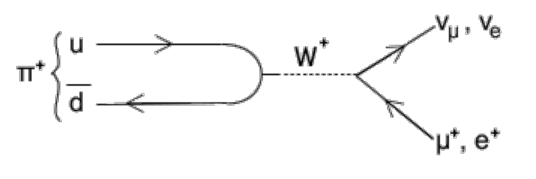
\includegraphics[width=.5\textwidth]{imgs/ep5-fig-8-8.pdf}
\caption{Helizitätsverletzung im $\pi^+$-Zerfall \label{fig:8.8}}
\end{figure}

\begin{align*}
\frac{\Gamma \lb  \pi^+ \ra e^+ \nu_e\rb }{\Gamma \lb  \pi^+ \ra \mu^+ \nu_\mu\rb  }= 1.2\cdot 10^{-4}
\end{align*}
Warum? Phasenraumfaktor ist viel größer für $\pi^+ \ra e^+ \nu_e$, weil $m_e\ll m_\mu$

\begin{figure}[!ht]
\centering
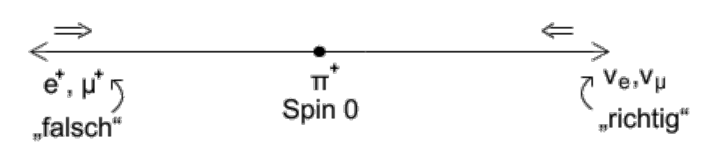
\includegraphics[width=.5\textwidth]{imgs/ep5-fig-8-9.pdf}
\caption{falsche Helizität für $e$, $\mu$ \label{fig:8.9}}
\end{figure}
\newpage

\begin{itemize}
\item[$\lt$] $\nu$ muss $h=-1$ haben
\item[$\lt$] $e$, $\mu$ muss $h=-1$ haben (Drehimpulserhaltung)
\begin{itemize}
\item[$\Ra$] $e$, $\mu$ hat \glqq falsche\grqq{} Helizität
\item[$\Ra$] unterdrückt mit $\frac{1 - \beta}{2}$\\
Faktor:
\begin{align}
\frac{m_e^2}{\lb M_\pi + m_e\rb ^2} \ll \frac{\mu_\mu^2}{\lb M_\pi + m_\mu \rb ^2}
\end{align}

\begin{align*}
\Gamma \lb  \pi^+ \ra e^+ \nu_e\rb  \ll \Gamma \lb  \pi^+ \ra \mu^+ \nu_\mu\rb 
\end{align*}
\end{itemize}
\end{itemize}
\end{itemize}

\section{CP-Symmetrie und CP-Verletzung}
\begin{itemize}
\item \tb{Erinnerung:}\\
$\hat{C}$ = Ladungskonjugation
\begin{align*}
\hat{C} \ket{\Psi} = \pm \ket{\bar{\Psi}}\\
\hat{C}\ket{\pi^0} = + \ket{\pi^0}\\
\hat{C}\ket{\pi^+ \pi^-} = \lb -1\rb ^2 \ket{\pi^+ \pi^-}
\end{align*}
\item \tb{CP-Transformation}
\begin{align}\begin{split}
\hat{C}\hat{P} \ket{\pi^0} = - \ket{\pi^0} \hspace*{1cm} (J^\mr{PC} = 0^{-+})\\
\hat{C}\hat{C} \ket{\gamma} \hspace*{1cm} (J^\mr{PC} = 0^{--})\\
\hat{C}\hat{P} \ket{\pi^+\pi^-} = (-1)^L \ket{\pi^+ \pi^-} \overset{\text{alle }L=0}{=} - \ket{\pi^+ \pi^-\pi^0}
\end{split}\end{align}
\newpage

\item \tb{$\hat{C}$- und $\hat{P}$-Transformatioen von Neutrinos}

\begin{figure}[!ht]
\centering
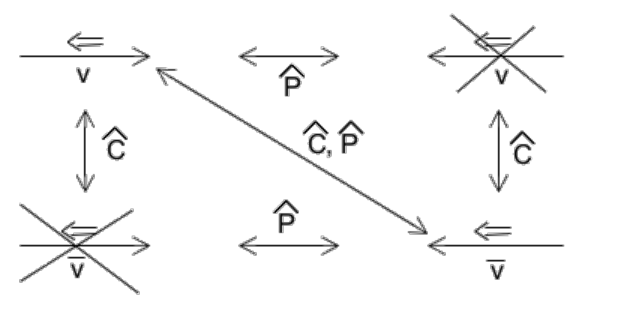
\includegraphics[width=.65\textwidth]{imgs/ep5-fig-8-10.pdf}
\caption{Skizze zur $C$- und $P$-Transformation \label{fig:8.10}}
\end{figure}

\begin{itemize}
\item[$\Ra$] $C$ ist maximal verletzt (wie $P$)
\item[$\Ra$] $CP$ könnte erhalten sein (fester \glqq Glaube\grqq{} bis 1964)
\end{itemize}
\item \tb{Entdeckung der $CP$-Verletzung} 1964 im $K^0$-System
\begin{align*}
\lno \begin{matrix}
\ket{K^0} = \ket{d\bar{s}}\\ \ket{K^0} = \ket{ s\bar{d}}
\end{matrix}\rrb\text{ können sich ineinander umwandeln}
\end{align*}

\begin{figure}[!ht]
\centering
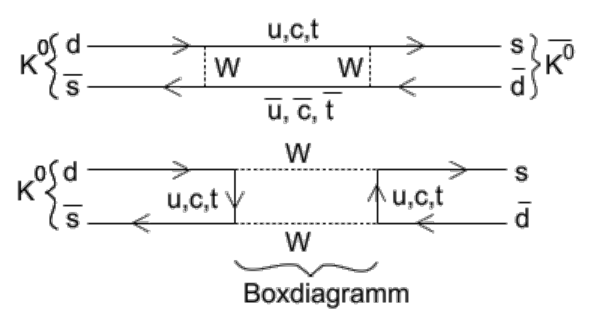
\includegraphics[width=.5\textwidth]{imgs/ep5-fig-8-11.pdf}
\caption{Möglichkeiten zur $K^0$-Umwandlung \label{fig:8.11}}
\end{figure}

\begin{itemize}
\item[$\Ra$] Beobachtet werden $K^0$-$\bar{K}^0$-Mischungen
\item[$\Ra$] Konstruiere $CP$-Eigenzustände
\begin{align}
\lno \begin{matrix}
\hat{C} \ket{K^0} = \ket{\bar{K}^0}\\
\hat{P} \ket{K^0} = - \ket{K^0}
\end{matrix}\rrb \hat{C}\hat{P} \ket{K^0} = - \ket{\bar{K}^0}\nonumber \\
\lno \begin{matrix}
\hat{C} \ket{\bar{K}^0} = \ket{K^0}\\
\hat{P} \ket{\bar{K}^0} = - \ket{\bar{K}^0}
\end{matrix}\rrb \hat{C}\hat{P} \ket{\bar{K}^0} = - \ket{K^0}\nonumber \\
\boxed{\begin{matrix}
\ket{K_1} = \frac{1}{\sqrt{2}} \lb  \ket{K^0} - \ket{\bar{K}^0} \rb , & \hat{C}\hat{P} \ket{K_1} = \ket{K_1}\\
\ket{K_2} = \frac{1}{\sqrt{2}} \lb  \ket{K^0} + \ket{\bar{K}^0}\rb , & \hat{C}\hat{P}\ket{K_2} = - \ket{K_2}
\end{matrix}}
\end{align}
Wenn $CP$ erhalten.\\
$K_1$ zerfällt in $CP$-Eigenzustand mit $CP=+1$\\
$K_2$ zerfällt in $CP$-Eigenzustand mit $CP=-1$\\
Insbesondere:
\begin{align*}
K_1 \ra 2\pi \hspace*{1cm} &\lb \tau_1 = 0.9 \cdot 10^{-10}\,\mr{s}\rb \\
K_2 \ra 3 \pi \hspace*{1cm} &\underbrace{\lb  \tau_2 = 5.1\cdot 10^{-8}\mr{s}\rb }_{\substack{\text{Phasenraumeffekt}\\lb M_n - 2M_\pi \gg M_n - 3M_\pi)}}
\end{align*}
\tb{Experiment:}
\begin{figure}[!ht]
\centering
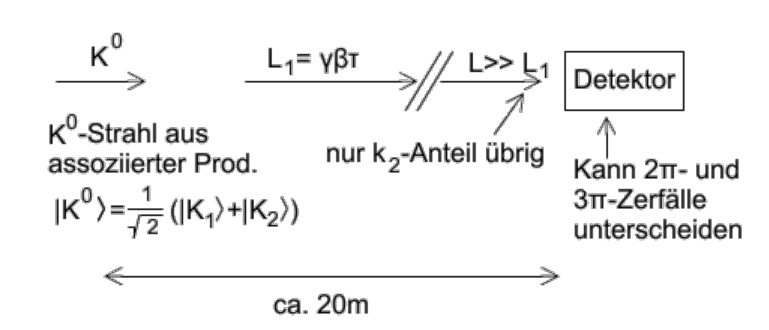
\includegraphics[width=.5\textwidth]{imgs/ep5-fig-8-12.pdf}
\caption{Skizze zum experimentellen Aufbau \label{fig:8.12}}
\end{figure}

Ergebnis:
\begin{align}
& \boxed{ K_2 \ra 2\pi \text{ mit } 0.23\,\% \text{ WS}}\\
& \Ra \ CP\text{-Verletzung}\nonumber
\end{align}
\item[$\lt$] $CP$-Verletzung auch in $B$- und $C$-Systemen
\item[$\lt$] $K^0$-Eigenzustände der schwachen WW:
\begin{align*}
\boxed{ \begin{matrix}
\ket{K_S} = \frac{1}{\sqrt{1+\epsi^2}} \lb  \ket{K_2} + \epsi \ket{K_1}\rb \\
\ket{K_L} = \frac{1}{\sqrt{1+\epsi^2}} \lb  \ket{K_1} - \epsi \ket{K_2}\rb 
\end{matrix}}
\end{align*}
Hierbei $S$ = Short, $L$ = Long und $\epsi = 0.0023$
\item[$\Ra$] $CP$-Verletzung bricht Symmetrie zwischen Materie und Antimaterie.\\
Aber: gemessener Effekt zu klein, um Materie Überschuss im Universum zu erklären.
\item[$\Ra$] Gemessene $CP$-Verletzung kann erklärt werden durch komplexe Phase in $CKMM$
\end{itemize}
\end{itemize}


\section{Neutraler Strom und Z-Boson}

\begin{itemize}
\item[$\lt$] $Z$-Austausch:

\begin{figure}[!ht]
\centering
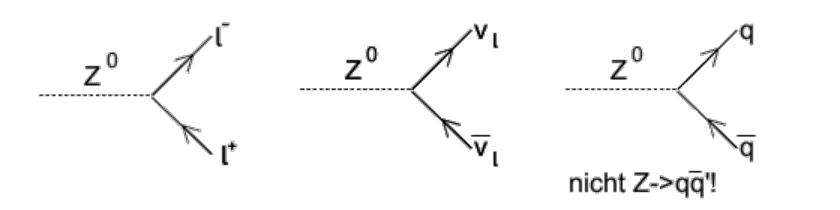
\includegraphics[width=.5\textwidth]{imgs/ep5-fig-8-13.pdf}
\caption{Möglichkeiten des $Z$-Austausches \label{fig:8.13}}
\end{figure}

\item[$\lt$] Kopplungsstärke:
\begin{align}
\boxed{g_Z = \frac{g_W}{\cos \theta_W} = \frac{e}{\sin \theta \cos \theta}}
\end{align}
\item[$\lt$] Wenn keine $\nu$'s beteiligt sind, sind $Z^0$- und $\gamma$-Austausch beide möglich (vgl. Abb.\ref{fig:8.14}).

\begin{figure}[!ht]
\centering
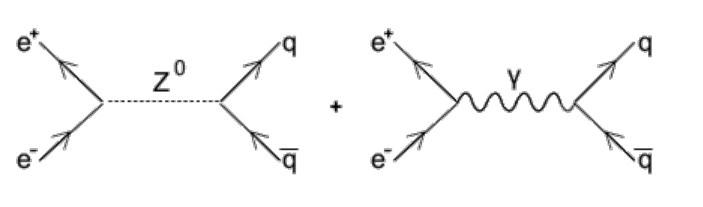
\includegraphics[width=.5\textwidth]{imgs/ep5-fig-8-14.pdf}
\caption{Beispiel zum $Z$- und $\gamma$-Austausch \label{fig:8.14}}
\end{figure}

\begin{align*}
\Ra \ \sigma, \Gamma \sim \labs \mc{M}_Z + \mc{M}_\gamma \rabs^2
\end{align*}
\begin{itemize}
\item[$\Ra$] Interferenzterme, Unterscheidung $Z$- und $\gamma$-Austausch ist für einzelne Prozesse nicht möglich
\item[$\Ra$] Bei $Q^2 \ll M_Z^2$ dominiert $\gamma$-Austausch
\end{itemize}
\item[$\lt$] $Z$ koppelt an $\ket{\Psi_L}$ und $\ket{\Psi_R}$ (ladungsabhängig)\\
$Z$ koppelt nur an $\nu_L$, $\bar{\nu}_R$
\item[$\lt$] $Z$-Quark-Kopplungen:\\
\glqq Algebraisch\grqq{}
\begin{align*}
\begin{pmatrix}
d^\prime\\ s^\prime \\ b^\prime
\end{pmatrix}^\top \ \ \begin{pmatrix}
d^\prime \\ s^\prime \\ b^\prime
\end{pmatrix} = \begin{pmatrix}
d\\ s\\ b\end{pmatrix}^\top \underbrace{U_\mr{CMK}^\dagger U_\mr{CMK}}_{\mb{1}_3} \begin{pmatrix}
d \\ s\\ b
\end{pmatrix} = \begin{pmatrix}
d \\ s \\ b 
\end{pmatrix}^\top \begin{pmatrix}
d \\ s\\ b
\end{pmatrix}
\end{align*}
$\Ra$ \tb{Keine} \glqq Flavour-changing neutral currents\grqq{} (FCNC)

\begin{figure}[!ht]
\centering
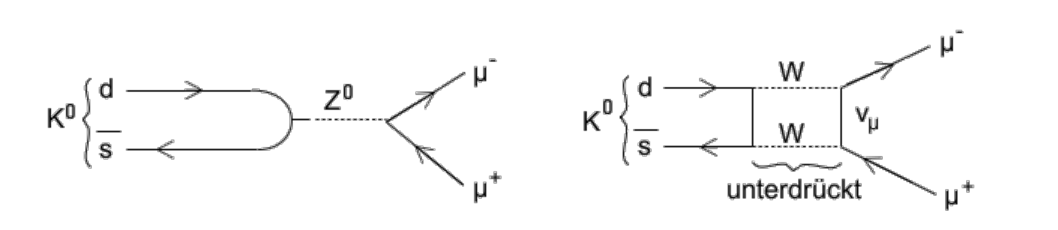
\includegraphics[width=.5\textwidth]{imgs/ep5-fig-8-15.pdf}
\caption{Beispiel des Zerfalls $K^0 \ra \mu^+ \mu^-$ mit Branchingratio $BR=1.5\times 10^{-6}$ \label{fig:8.15}}
\end{figure}

\dots weil $\underbrace{\sim V_{du} V_{su}^\star + V_{dc}V_{sc}^\star + V_{dt}V_{st}^\star}_\text{Elemente der $CKMM$} =0$\\
(der sog. GIM-Mechanismus: Glashow, Iliopoulos, Maiami)\\
\dots trotzdem möglich, weil $m_u \ll m_c \ll m_t$
\end{itemize}

\section{Direkte Produktion von \texorpdfstring{$W$}- und \texorpdfstring{$Z$}-Bosonen}
\begin{itemize}
\item \tb{Geschichte:}
\begin{itemize}
\item[1968:] Theorie der elktroschwachen Wechselwirkung (Glashow, Weinberg, Salam Nobel-Preis 1979)
\item[1973:] Erster Nachweis von Reaktionen mit $Z$-Austausch ($\nu A \ra \nu A$, CERN)
\item[1983:] Direkter Nachweis von $Z,\ W$ (CERN) (NP 1984: Rubbia, van der Meer)
\item[199er:] $Z$-Präzisionsmessungen (CERN) 
\end{itemize}
\item \tb{Entdeckung von $W$ und $Z$}\\
$p - \bar{p}$-Collider Sp$\bar{\mr{p}}$S, CERN
\item \tb{$W$-Erzeugung}

\begin{figure}[!ht]
\centering
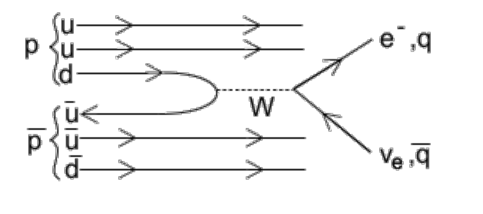
\includegraphics[width=.5\textwidth]{imgs/ep5-fig-8-16.pdf}
\caption{$W$ Erzeugung bei Wechselwirkung von Proton und Antiproton \label{fig:8.16}}
\end{figure}

\glqq Reste\grqq{} von $p$ und $\bar{p}$ (also $uu$ und $\bar{u}\bar{d}$) bilden Jets im Strahlrohr.\\
Das $W$ hat einen Impuls $E_p \lb xd - x\bar{u}\rb $ in Strahlrichtung
\item \tb{$W$-Zerfall:}
\begin{align*}
\begin{matrix}
\text{leptonisch } & \llb \begin{matrix} W^\pm \ra & e^+ \nu_e, e^- \bar{\nu}_e\\ & \mu^+ \nu_\mu, \mu^- \bar{\nu}_\mu\\ &\tau^+ \nu_\tau, \tau^- \bar{\nu}_\tau \end{matrix} \rrb & \text{ je 10.9\,\% (Lepton-Universalität)}\\ & & \\
\text{hadronisch } & W^\pm$ $\ra\ \underbrace{q \bar{q}^\prime}_{ud^\prime, cs^\prime} \ra  2\text{ jets} & 67.2\,\%
\end{matrix}
\end{align*}

$ud^\prime,\ cs^\prime$ schwache EZ, 3 mögliche Farben. Somit $2 \cdot 3 \cdot 11.2\,\%$\\
-- Achtung: $W^\pm \ra t+x,\bar{t}+x$ verboten wegen $m_t > M_W$
\item[$\ra$] \tb{$W$-Identifikation}\\
Zuerst in leptonischen Zerfällen
\begin{itemize}
\item \glqq missing $p_T$\grqq{} von $\nu$
\item einzelne Teilchenspur $(e)$
\item charkteristisches Signal im Kalorimeter $(e)$
\end{itemize}
\item[$\ra$] \tb{$W$-Eigenschaften}\\
$M_W= 80.385$\,GeV, $\Gamma_W = 2.085$\,GeV, $\tau = 3\times 10^{-25}$\,s
\item \tb{$Z$-Erzeugung: Wie $W$}

\begin{figure}[!ht]
\centering
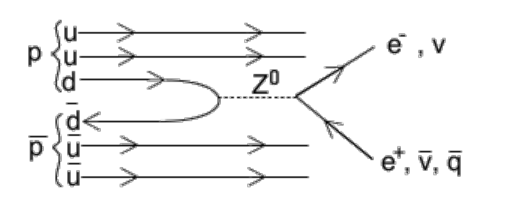
\includegraphics[width=.5\textwidth]{imgs/ep5-fig-8-17.pdf}
\caption{$Z$-Erzeugung bei Proton-Antiproton-Streuung\label{fig:8.17}}
\end{figure}

\item \tb{$Z$-Zerfall}
\begin{align*}
\begin{matrix}
\text{leptonisch } & \llb Z^0 \ra  \begin{matrix}
\lno\begin{matrix}
e^+e^-\\ \mu^+\mu^- \\ \tau^+ \tau^-
\end{matrix}\rrb &\text{ je 3.4\,\% (Lepton-Universalität)}\\
\lno\begin{matrix}
\nu \bar{\nu}\\ \text{(invisible)\grqq{}}
\end{matrix}\rrb & 20\,\%
\end{matrix}\rno \\
\text{hadronisch: } & Z^0 \ra q\bar{q}\ \ra 2\text{ jets}\qquad \qquad \qquad 69.9\,\% \qquad \qquad
\end{matrix}
\end{align*}

$q\bar{q} = d\bar{d},u\bar{u},s\bar{s},c\bar{c},b\bar{b},\text{ nicht } t\bar{t}$
\item \tb{$Z$-Eigenschaften}\\
$M_Z = 91.1876$\,GeV, $\Gamma = 2.4952$\,GeV, $\tau \approx 2\times 10^{-25}$\,s
\item \tb{Präzisionsmessung des $Z$}\\
LEP: $e^+e^-$-Collider, CERN

\begin{figure}[!ht]
\centering
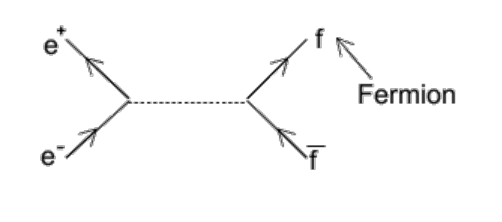
\includegraphics[width=.5\textwidth]{imgs/ep5-fig-8-18.pdf}
\caption{$e^+e^-$-WW mit Fermion-Antifermionenpaar \label{fig:8.18}}
\end{figure}

wenn $\Gamma_s = M_Z$ (d.h.$E_{e^-} = E_{e^+} = \frac{M_Z}{2}$) $\Ra$ $Z$ ruht im Laborsystem\\
WQ bei $\Gamma_s = M_Z$ ist groß, aber endlich. (Warum endlich?)
\begin{itemize}
\item $Z$ instabil
\begin{align}
\Psi_Z \sim e^{iM_Z} e^{-\frac{\Gamma_s t}{2}}
\end{align}
\item Im Propagator:
\begin{align}
 M_z \ra M_Z - i \frac{\Gamma_Z}{2}\\
 \Ra \labs \frac{1}{S-M_Z^2}\rabs^2 \ra \labs \frac{1}{S- M_Z^2 + i \frac{\Gamma_Z}{2} M_Z}\rabs\\
 = \frac{1}{\lb S- M_Z^2\rb ^2 + M_Z^2 \Gamma_Z^2}
\end{align}
$\Ra$ WQ $\lb e^+e^-\ra Z\rb $ hat Resonanz bei $\Gamma_S = M_Z$

\begin{figure}[!ht]
\centering
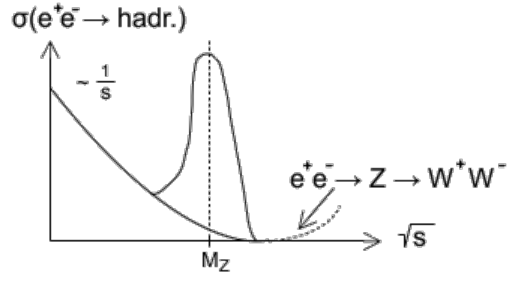
\includegraphics[width=.5\textwidth]{imgs/ep5-fig-8-19.pdf}
\caption{Diagramm zur $M_Z$-Resonanz \label{fig:8.19}}
\end{figure}


Bei LEP: $\sim 2 \times 10^7$ $Z$-Ereignisse (4 Experimente)\\
Bei SLAC: $\sim0.5\times 10^6$ $Z$-Ereignisse mit polarisierten $e^+, \ e^-$ (1 Experiment)
\item Präzisionsmessung der $Z$-Resonanz
\item Genaue Messung der elektroschwachen Parameter:\\
z.B. $M_Z$, $\Gamma_Z$, $\sin \theta_W$, Kopplungen, \dots
\begin{itemize}
\item[$\Ra$] $\boxed{\text{Alle Ergebnisse im Einklang mit dem Standardmodell}}$
\item[$\Ra$] Test von höheren Ordnungen!
\item[$\ra$] Besipiel: Bestimmung der Zahl leichter $\nu$-Flavours aus $\Gamma_Z$:
\begin{align}
\Aboxed{\Gamma_Z = \Gamma_\mr{had} + \Gamma_e + \Gamma_\mu + \Gamma_\tau + \underbrace{\Gamma_\nu}_{\sim N \nu}}
\end{align}
Messung von $\Gamma_Z$ aus:
\begin{align}
\Aboxed{\sigma_\mr{had} = \sigma\lb e^+e^- \ra \text{Hadronen}\rb   = A \cdot \frac{S}{\lb S-M_Z^2\rb ^2 + M_Z^2 \Gamma_Z^2}}
\end{align}
$A$ aus Theorie bekannt\\
$S$ von Beschleuniger\\
$M_Z$ von Resonanz-Maximum\\
$\lt$ $\sigma_\mr{had} \lb  \Gamma_S = M_Z \rb  \sim \frac{1}{\Gamma_Z^2}$\\
$\lt$ $\Gamma_S \approx M_Z$ mit MeV-Genauigkeit gemessen ($\Ra$ erfordert Korrekturen auf Gezeiten, Wasserstand in Genfer See, Züge, \dots )\\
$\lt$ Ergebnis:
\begin{align}
\Aboxed{N_\nu = 2.984 \pm 0.08}
\end{align}
\item Nicht besprochen: Strahlungskorrekturen

\begin{figure}[!ht]
\centering
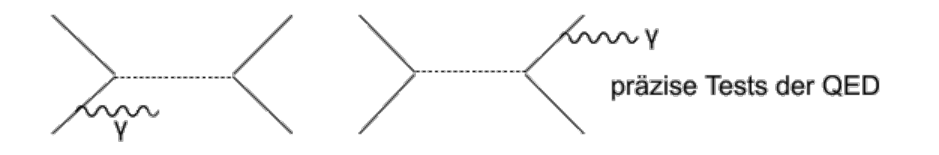
\includegraphics[width=.65\textwidth]{imgs/ep5-fig-8-20.pdf}
\caption{Feynmandiagramm zu Nebenstrahlungen, die korrigiert werden müssen \label{fig:8.20}}
\end{figure}

$\lt$ berechnet mit QED
\end{itemize}
\end{itemize}
\item \tb{$e^+e^- \ra W^+W^-$}\\
LEP-Energie erhöht auf $\sim 110$\,GeV $\Ra \ e^+e^-\ra \underbrace{W^+W^-}_\text{reell}$ möglich

\begin{figure}[!ht]
\centering
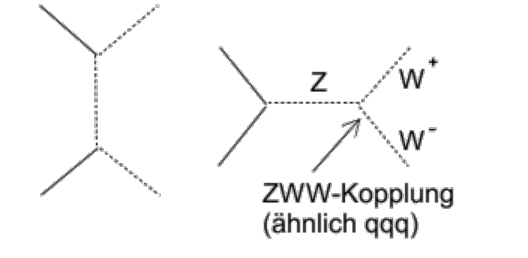
\includegraphics[width=.5\textwidth]{imgs/ep5-fig-8-21.pdf}
\caption{Feynmandiagramm zur Wechselwirkung von $e^+e^- \ra W^+W^-$ über ein $Z$-Boson\label{fig:8.21}}
\end{figure}

Ergebnis: beide Graphen erforderlic!ht
\end{itemize}
